\section{Studio del dominio}

%TODO Riempire di citazioni

\subsection{Il fallimento}
Il fallimento è lo strumento attraverso il quale si supera l'inattività o la volontà contraria al soddisfacimento delle obbligazioni assunte dal debitore, rispetto alle quali il suo intero patrimonio svolge una funzione di garanzia.

Si svolge nell'interesse dei creditori e nel rispetto della par condicio creditorum innanzi al Tribunale del luogo ove ha sede principale l'imprenditore.

Lo stato d'insolvenza si manifesta con inadempimenti o altri fatti esteriori, i quali dimostrino che il debitore non è più in grado di soddisfare regolarmente le proprie obbligazioni.

\subsection{Soggetti interessati}

\subsubsection{Tribunale fallimentare}
L'organo principale investito dell'intera procedura fallimentare. Nomina, revoca e sostituisce gli altri organi della procedura, quando non è prevista la competenza del giudice delegato.

\subsubsection{Imprenditore}
Sono soggetti alle disposizioni sul fallimento gli imprenditori che esercitano un'attività commerciale.

\subsubsection{Giudice delegato}
Il giudice delegato esercita funzioni di vigilanza e di controllo sulla regolarità della procedura.

\subsubsection{Curatore fallimentare}
Il curatore fallimentare è colui che ha l’amministrazione del patrimonio fallimentare e compie tutte le operazioni della procedura fallimentare sotto la vigilanza del giudice delegato e del comitato dei creditori, nell’ambito delle funzioni ad esso attribuite.


\subsubsection{Comitato dei creditori}
Il comitato dei creditori vigila sull'operato del curatore e ne propone la revoca, autorizza gli atti, esprime pareri.
I membri possono svolgere ispezioni sulle scritture contabili e sui documenti della procedura. È nominato dal giudice delegato, sentiti il curatore e i creditori stessi.


\subsection{Istanza di fallimento}
L’istanza di fallimento è l’atto attraverso il quale viene richiesto alla Pubblica Autorità di aprire una procedura fallimentare nei confronti di un determinato imprenditore.

Può essere presentata da:
\begin{itemize}
\item il debitore stesso che chiede il proprio fallimento; 
\item i creditori di un soggetto insolvente; 
\item il pubblico ministero. 
\end{itemize}

\subsection{Iscrizione al passivo}
Qualunque soggetto sia creditore di un imprenditore fallito ha diritto ad insinuarsi al passivo del fallimento, così da poter concorrere, insieme agli altri creditori insinuati, per ottenere il soddisfacimento del proprio credito nell'ambito del fallimento.

\subsubsection{Tipologia di iscrizione}
\label{Tipologia di iscrizione}
Se il credito è assistito da un privilegio (come ad esempio il pegno o l’ipoteca) ha diritto ad essere soddisfatto con precedenza sugli altri creditori non privilegiati; se invece non è assistito da privilegio si dice creditore "chirografario", il cui credito può essere soddisfatto solo e nella misura in cui vi sia un residuo dell'attivo fallimentare dopo il soddisfacimento dei creditori privilegiati. 
Con la domanda di ammissione al passivo, quindi, il creditore presenta agli organi del fallimento la propria domanda di insinuazione al passivo, ovvero di essere incluso nel novero dei creditori che concorreranno alla distribuzione dell'attivo del fallimento.

\subsubsection{Modelli di iscrizione al passivo}

%TODO controllare che le immagini stiano sotto il titolo.

\begin{figure}[h!tbp]
\centering
\fbox{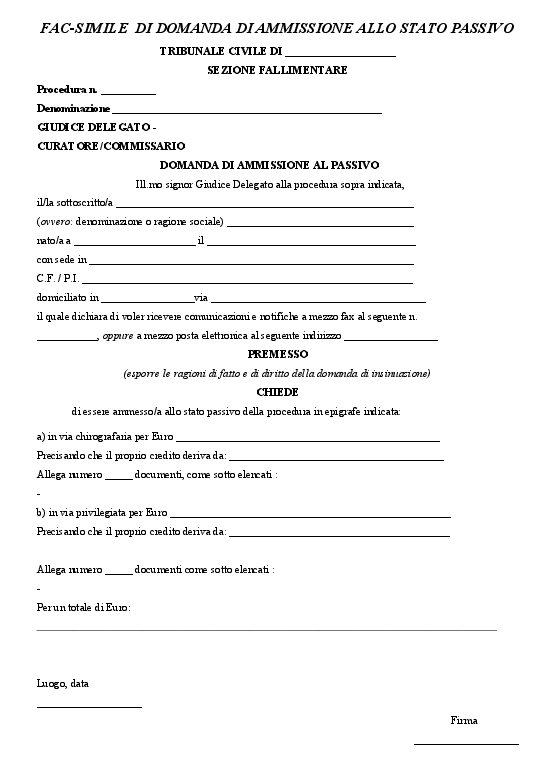
\includegraphics[width=.9\textwidth]{img/2.png}}
\caption{Fac-simile di domanda di ammissione allo stato passivo.}
\end{figure}

\begin{figure}[h!tbp]
\centering
\fbox{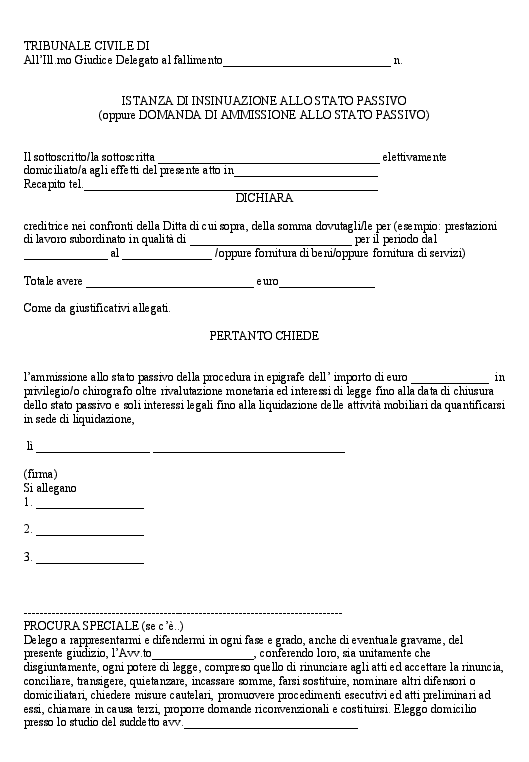
\includegraphics[width=.9\textwidth]{img/3.png}}
\caption{Istanza di insinuazione allo stato passivo.}
\end{figure}

\begin{figure}[h!tbp]
\centering
\fbox{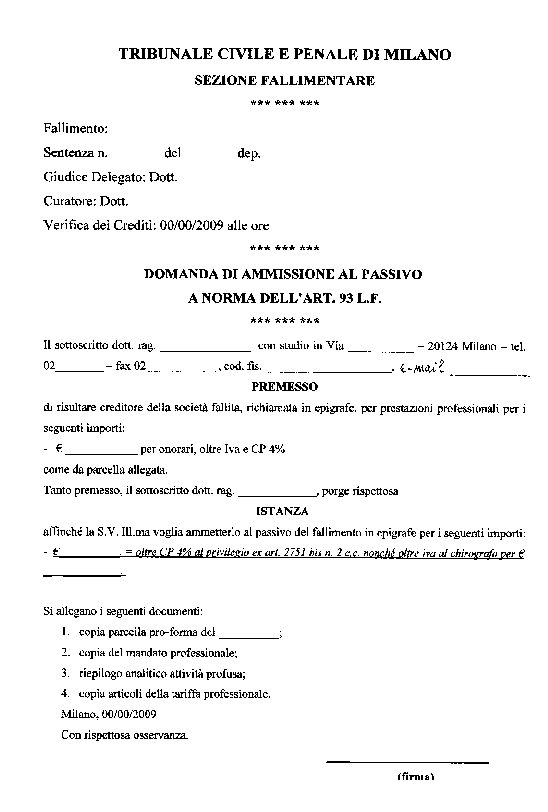
\includegraphics[width=.9\textwidth]{img/1.png}}
\caption{Modello di iscrizione al passivo pubblicato online dal Tribunale di Milano.}
\label{fig:ModelloMilano}
\end{figure}


\subsection{Individuazione dei bisogni dell’utente}
A causa della scarsa informatizzazione dei Tribunali (come purtroppo della maggior parte delle strutture pubbliche in Italia), i moduli da presentare ad ogni livello della procedura sono in forma cartacea, basati su modelli spesso diversi tra loro.

Ad esempio, la fig.~\ref{fig:ModelloMilano} mostra il modello pubblicato e liberamente scaricabile dal sito del Tribunale Civile e Penale di Milano \cite{milano:modulistica}.

Come è facile intuire, la presenza di diversi modelli, unita al numero elevato di documenti da esaminare, rende oneroso il compito del curatore fallimentare.

Per semplificare il lavoro sarebbe utile uno strumento in grado di estrarre in maniera automatica le informazioni necessarie al curatore, indipendentemente dal template utilizzato.

